% 第六章：实验评估——Zen 4 百万级真实与合成双曲基准、表示对照、外部系统表格、多线程扩展、消融实验与四阶段召回损失分解
\section{Experimental Evaluation}
\label{sec:eval}

We evaluate native hyperbolic retrieval on {MERU-1M} and {WordNet-Hazy}, and use mapped {Cohere-1M} and {OpenAI-1536} to measure high-dimensional shell behavior. The same-graph controls separate the costs of graph traversal, page layout and cold reranking. A deeper native {WordNet} embedding and four synthetic geometries let us vary directional concentration and depth beyond the range of {MERU-1M}.

\subsection{Experimental Setup}
\label{subsec:eval_setup}

\paragraph{Hardware and Protocol.}
Experiments run in isolated Linux containers with {AMD EPYC 9654} ({Zen~4}) CPUs, each restricted via cgroups to 32 logical CPUs and $60$\,GiB RAM. Swap is disabled and transparent huge pages ({THP}) are set to \texttt{never}, using standard $4$\,KiB pages for {DTLB} translation. Each instance runs one timed benchmark at a time, and measurement manifests record instance placement and source/binary fingerprints.
All Rust binaries are compiled in release mode targeting native {AVX-512F} and {AVX2+FMA}.
Unless otherwise stated, graph indices use base degree $M = 16$ (maximum out-degree $M_0 = 32$), construction beam $L_c = 128$, geodesic slack $\alpha = 1.2$, and $32$ build threads.
Following community {ANN} protocols~\cite{aumuller2020annbenchmarks,simhadri2022results}, the throughput tables and frontier curves use one build per configuration (seed \texttt{12345} where supported, upstream randomization for HDB). We also checked three seeds (\texttt{12345}, \texttt{12446}, \texttt{12547}) for sensitivity to construction.
Across three seeds, the largest within-configuration Recall@10 range was $0.220$ percentage points over 352 settings on {Cohere-1M}, {MERU-1M} and {OpenAI-1536}, and $0.695$ points over 62 synthetic settings (on {Uniform-Narrow}). At fixed $(L,B,\Delta_0)=(208,64,0.12)$, {\rquiver{}-Core} served $1{,}984$--$2{,}020$\,QPS on {Cohere-1M} at 1T. At $(128,128,0.20)$ it served $2{,}592$--$2{,}602$\,QPS on {MERU-1M}.
Each thread count selects the fastest qualifying measured operating point. Repeated-build diagnostics use the same seeds for all variants.

\paragraph{Fixed Parameters and Operating-Point Selection.}
Table~\ref{tab:fixed_parameters} gives the shared construction, cone-purity, and uncertainty settings. The full-method sweep uses
\[
 \begin{aligned}
 L\in\{&32,64,96,128,192,200,208,\\
       &256,384,512,768,1024,1536,2048\},
 \end{aligned}
\]
rerank budgets $B\in\{32,64,128\}$ subject to $B\le L$, and sketch margins $\Delta_0\in\{0.08,0.12,0.20\}$. Controlled engine sweeps additionally include full-pool reranking and sketch-disabled paths. Each query-thread count uses its measured qualifying operating points.
{MERU-1M}, {OpenAI-1536}, {WordNet-Hazy}, and the synthetic datasets use disjoint $2{,}000$-query tuning sets. For {Cohere-1M}, we use the $1{,}000$ public {VectorDBBench} queries and compute exact top-10 neighbors over the mapped database in FP64. For each method and thread count, the {Cohere-1M} frontier reports the highest measured QPS meeting each recall threshold on these queries.

\begin{table}[t]
  \centering
  \caption{Hyperbolic benchmarks in $\Bunit$ ($c=1$).}
  \label{tab:datasets}
  \small
  \setlength{\tabcolsep}{3.5pt}
  \begin{tabularx}{\linewidth}{@{}lrrr>{\raggedright\arraybackslash}X@{}}
    \toprule
    \textbf{Dataset} & $N$ & $D$ & $|Q|$ & \textbf{Manifold Geometry} \\
    \midrule
    Cohere-1M & 1,000K & 768 & 1,000 & Mapped Wikipedia (base $\rho_{0.01}=1.45$) \\
    MERU-1M~\cite{astrmira2026meruimagenet1m} & 1,000K & 512 & 10,000 & Native {Lorentz}$\to\Bunit$ multimodal \\
    OpenAI-1536 & 990K & 1,536 & 8,000 & Mapped DBpedia ($\exp_0^1$, $\text{med}\,\rho=2.0$) \\
    WordNet-Hazy & 83.9K & 20 & 2,000 & Native {Lorentz}$\to\mathbb{B}_1^{20}$ taxonomy \\
    \midrule
    Uniform-Narrow & 1,000K & 512 & 2,000 & Isotropic $\mathbb{S}^{511}$, $\rho \in [3.9, 4.1]$ \\
    Uniform-Wide & 1,000K & 512 & 2,000 & Isotropic $\mathbb{S}^{511}$, $\rho \in [0.4, 6.0]$ \\
    Clustered-Narrow & 1,000K & 512 & 2,000 & $256$ tight cones, $\rho \in [3.9, 4.1]$ \\
    Clustered-Wide & 1,000K & 512 & 2,000 & $256$ tight cones, $\rho \in [0.4, 6.0]$ \\
    \bottomrule
  \end{tabularx}
\end{table}

\paragraph{Benchmarks.}
Table~\ref{tab:datasets} summarizes the eight hyperbolic benchmarks in $\Bunit$ ($c=1$).
For Euclidean embeddings mapped into $\Bunit$, both \textbf{Cohere-1M} and \textbf{OpenAI-1536} use the origin exponential map from centered coordinates: given database mean $\bar{x}$ and global radial scale $s = 2 / \operatorname{median}_i(\|x_i - \bar{x}\|_2)$, each vector is mapped as
\[
\Phi(x) = \tanh\!\left(\frac{s}{2}\|x - \bar{x}\|_2\right)\frac{x - \bar{x}}{\|x - \bar{x}\|_2},
\]
clamped at Euclidean radius $1 - 10^{-6}$ so that the database median geodesic depth is fixed at $\rho_{0.50} = 2.0$.
On \textbf{Cohere-1M} (1M 768D Wikipedia embeddings, $1{,}000$ test queries, $s = 0.2644$, zero clipped vectors), norm concentration after mean-centering narrows base depths to $[0.98, 3.39]$ ($\rho_{0.01} = 1.45$, $\rho_{0.99} = 2.69$) and query depths to $[1.25, 2.98]$ ($\rho_{0.01} = 1.44$, $\rho_{0.99} = 2.67$), forming a hollow shell with minimum database depth $0.9776$.
\textbf{OpenAI-1536} applies unit $\ell_2$-normalization before mean-centering and $\Phi(x)$ ($s = 2.093$) across 990K 1536D \texttt{text-embedding-3-large} {DBpedia} embeddings with $8{,}000$ held-out test queries and $2{,}000$ tuning queries.
To evaluate native hyperbolic search at million-vector scale, we constructed and released \textbf{MERU-1M}~\cite{astrmira2026meruimagenet1m} by encoding {ImageNet} images with the frozen {MERU ViT-small} encoder~\cite{desai2023meru}.
The release includes the original Lorentz spatial coordinates, the preparation scripts, and canonical Poincar\'e coordinates for one million 512-dimensional training images and disjoint sets of $2{,}000$ tuning and $10{,}000$ test queries from the validation split. Rescaling the Lorentz spatial coordinates by $\sqrt{c}$ for model curvature $-c$ ($c\simeq0.1$) before applying~\eqref{eq:lorentz_isometry} scales all distances by the same factor $\sqrt{c}$ in exact arithmetic. Exhaustive FP64 ground truth uses the released FP32 ball coordinates.
\textbf{WordNet-Hazy} adapts the public $20$D native {Lorentz} {WordNet} weights (\texttt{wordnet\_full.emb}, $83{,}943$ base nodes and $2{,}000$ disjoint test queries) isometrically into $\mathbb{B}_1^{20}$ ($\le 2.53\times 10^{-15}$ max numerical error).
Four 1M-vector 512D synthetic benchmarks cross directional geometry (isotropic $\mathbb{S}^{511}$ versus $256$ tight spherical cones) with radial depth support (narrow boundary shell $\rho \in [3.9, 4.1]$ versus wide hierarchy $\rho \in [0.4, 6.0]$).

\paragraph{Baselines.}
Within our engine family, we evaluate two orthogonal groups of controlled variants:
(1)~\emph{Representation and frozen-graph controls:} \textbf{Polar-FP32} and \textbf{Polar-SQ8} share \rquiver{}'s {QuadriPrune} topology and router while substituting unquantized FP32 or 8-bit scalar-quantized unit directions during both construction and search, whereas \textbf{SameGraph-FP32} and \textbf{SameGraph-SQ8} freeze the 2-bit-constructed graph and replace only the search-time directional representation to decouple graph quality from traversal speed (plotted as \textbf{FP32 (same graph)} and \textbf{SQ8 (same graph)} alongside 2-bit {SM} in Figure~\ref{fig:abl_repr}).
(2)~\emph{Cumulative 2-bit engine progression:} \textbf{\rquiver{}-Split} (split-array 2-bit {QuadriPrune} without chord-swap island repair, \texttt{HotSmPage} co-location, or \texttt{SymSketch256}) $\to$ \textbf{\rquiver{}-Core} (adding chord-swap repair, $4096$\,B single-page co-location, and \texttt{SymSketch256} under global 2-bit {SM}) $\to$ full \textbf{\rquiver{}} (further enabling purity-gated \texttt{ResidualConeDict} and adaptive \textsc{CJ-Gate} plateau expansion; in \S\ref{subsec:eval_synthetic}, \textbf{Global-SM} denotes the unrescued global-code baseline without \texttt{ResidualConeDict}, \textsc{CJ-Gate}, or variance-stabilized sketch margins).
Under the same hardware and FP64 ground-truth protocol, we use \textbf{Exact-RobustPrune}~\cite{subramanya2019diskann,prokhorenkova2022hyperbolic} ($M/L_c = 16/128, L \le 2{,}048$) to test exact geodesic {Vamana} pruning on the mapped hollow shell of {Cohere-1M}. On {MERU-1M} we isolate the pruning predicate using the matched two-bit engine in \S\ref{subsec:eval_ablation}. We also test
\textbf{HyperspaceDB} (\textbf{HDB}, \texttt{YARlabs/hyperspace-db} commit \texttt{89d0406}, native {AVX-512F} {Poincar\'e} {HNSW})~\cite{glukhota2026hyperspacedb} across FP32 and FP64 hyperbolic modes and dynamic/flat storage layouts (\textbf{HDB FP32 dynamic}, \textbf{HDB FP32 flat}, \textbf{HDB FP64 dynamic}, \textbf{HDB FP64 flat}),
and flat inner-product {HNSW} indices in \textbf{Faiss} (\texttt{faiss-cpu 1.16.0} \texttt{IndexHNSWFlat})~\cite{douze2024faiss}---tested with mean-centered {Lorentz} inner product (\textbf{Faiss centered IP}), unit-direction search with exact FP64 reranking (\textbf{Faiss direction}), and uncentered {Lorentz} inner product (\textbf{Faiss raw Lorentz-IP})---and \textbf{Milvus} ({Milvus Standalone 3.0.5} {HNSW})~\cite{wang2021milvus} (\textbf{Milvus centered IP}), building {HDB}/{Faiss}/{Milvus} at both $(M=16, L_c=128)$ and $(M=32, L_c=256)$ and scanning $18$ $ef$ values up to $4{,}096$. In this full-precision sweep HDB and Milvus return their native top-10. Faiss uses FP64 geodesic reranking for direction search and tests both native and reranked IP outputs. For Lorentz coordinates $(t,\mathbf{s})$, centered IP stores $(t_v-\bar t,\mathbf{s}_v)$ and queries with $(-t_q,\mathbf{s}_q)$, where $\bar t$ is the database mean time coordinate. Their dot product preserves Lorentz ordering up to the query-only offset $t_q\bar t$ before rounding. HNSW builds links using ordinary inner products between stored vectors. Raw IP sets the centering offset to zero.

\subsection{Index Construction and Polar Representation Comparison}
\label{subsec:eval_repr}

\begin{table*}[t]
  \centering
  \caption{Active navigation memory, build time and threshold throughput. Every method uses one build per construction configuration.}
  \label{tab:zen4_repr}
  \small
  \setlength{\tabcolsep}{3pt}
  \begin{tabular}{@{}llrrrrrrrrrrrr@{}}
    \toprule
    & & \textbf{Build} & \textbf{Hot Nav} & \textbf{Zero-In} & \multicolumn{3}{c}{\textbf{Recall@10 $\ge 98\%$}} & \multicolumn{3}{c}{\textbf{Recall@10 $\ge 99\%$}} & \multicolumn{3}{c}{\textbf{Recall@10 $\ge 99.5\%$}} \\
    \cmidrule(lr){6-8}\cmidrule(lr){9-11}\cmidrule(lr){12-14}
    \textbf{Dataset} & \textbf{Method} & \textbf{32T (s)} & \textbf{(MB)} & \textbf{Islands} & \textbf{1T QPS} & \textbf{p99} & \textbf{24T QPS} & \textbf{1T QPS} & \textbf{p99} & \textbf{24T QPS} & \textbf{1T QPS} & \textbf{p99} & \textbf{24T QPS} \\
    \midrule
    \multirow{7}{*}{Cohere-1M}
    & Polar-FP32 & 197.7 & 3,373.0$^\ddagger$ & 0 & 1,048 & 1.17 & 15,063 & 457 & 2.63 & 7,004 & 265 & 4.33 & 3,928 \\
    & Polar-SQ8 & 68.3 & 1,069.0 & 0 & 1,818 & 0.75 & 36,304 & 858 & 1.56 & 16,488 & 396 & 3.25 & 7,353 \\
    & SameGraph-FP32 & 32.8 & 3,373.0$^\ddagger$ & 0 & 1,054 & 1.20 & \missing & 467 & 2.52 & \missing & 96 & 11.77 & \missing \\
    & SameGraph-SQ8 & 32.8 & 1,069.0 & 0 & 2,029 & 0.60 & \missing & 906 & 1.57 & \missing & 182 & 6.39 & \missing \\
    & \rquiver{}-Split & \textbf{32.2} & \textbf{485.0} & 628 & 2,765 & 0.43 & 56,828 & 1,739 & 0.72 & 37,747 & 617 & 1.84 & 14,393 \\
    & \rquiver{}-Core & 32.8 & 517.0 & 0 & \textbf{3,800} & \textbf{0.31} & \textbf{73,861} & \textbf{2,003} & \textbf{0.59} & \textbf{46,796} & 687 & \textbf{1.64} & 16,029 \\
    & \textbf{\rquiver{}} & 35.0 & 517.0$^*$ & \textbf{0} & 2,907 & 0.41 & 58,162 & 1,930 & 0.62 & 42,466 & \textbf{738} & 1.65 & \textbf{17,137} \\
    \midrule
    MERU-1M & \textbf{\rquiver{}} & \textbf{25.7} & \textbf{516.8}$^*$ & \textbf{0} & \textbf{2,547} & \textbf{0.50} & \textbf{53,483} & \textbf{2,547} & \textbf{0.50} & \textbf{53,483} & \textbf{1,669} & \textbf{0.81} & \textbf{36,092} \\
    OpenAI-1536 & \textbf{\rquiver{}} & \textbf{43.6} & \textbf{765.6}$^*$ & \textbf{0} & \textbf{1,378} & \textbf{1.03} & \textbf{25,725} & \textbf{792} & \textbf{1.81} & \textbf{14,731} & \textbf{481} & \textbf{3.05} & \textbf{9,094} \\
    WordNet-Hazy & \textbf{\rquiver{}} & \textbf{1.5} & \textbf{32.8}$^*$ & \textbf{0} & \textbf{4,130} & \textbf{0.29} & \textbf{89,847} & \textbf{3,089} & \textbf{0.38} & \textbf{65,405} & \textbf{2,341} & \textbf{0.49} & \textbf{52,371} \\
    \bottomrule
  \end{tabular}
  \par\vspace{2pt}
  {\footnotesize Latency is 1T p99 in ms. $^*$The page allocation includes the sketch and alignment. The split counters for full {Cohere}, {MERU}, {OpenAI} and {WordNet-Hazy} are $485.0$, $420.8$, $670.6$ and $26.1$\,MB. $^\ddagger$The active navigation total excludes the retained, unused 2-bit buffers in the two control formats (Table~\ref{tab:memory_audit}). }
\end{table*}

Table~\ref{tab:zen4_repr} evaluates controlled polar directional representations on {Cohere-1M} and summarizes end-to-end \rquiver{} performance across all four real hyperbolic workloads.

\paragraph{Construction Speed and Memory Footprint.}
On mapped {Cohere-1M}, \rquiver{} constructs a graph reachable from its entry hubs in $35.0$\,s on 32 threads, versus $197.7$\,s for {Polar-FP32} and $68.3$\,s for {Polar-SQ8}. Active navigation falls from $3{,}373$ to $517$\,MB relative to FP32 ($6.52\times$). The FP32 control also uses its traversal vectors for reranking. The 2-bit engine keeps a separate $3{,}072$\,MB cold store, bringing its accounted index total to $3{,}589$\,MB. At the $99.5\%$-target 1T points in Table~\ref{tab:zen4_repr}, process RSS is $3{,}939$\,MB for \rquiver{} and $3{,}879$\,MB for {Polar-FP32}. Table~\ref{tab:memory_audit} reconciles the index arrays.
On native {MERU-1M}, mapped {OpenAI-1536}, and native {WordNet-Hazy}, 32-thread construction takes $25.7$, $43.6$, and $1.5$\,s. All four primary real graphs have full entry reachability and zero retained cones.

\paragraph{Matched-Recall Throughput and Graph-Quality Crossover.}
At $\ge 99\%$ Recall@10 on {Cohere-1M}, \rquiver{} reaches \textbf{$1{,}930$\,QPS} ($0.62$\,ms p99) on 1 thread and \textbf{$42{,}466$\,QPS} ($1.20$\,ms p99) on 24 threads, improving over {Polar-FP32} by \textbf{$4.23\times$ (1T)} and \textbf{$6.06\times$ (24T)}, and over {Polar-SQ8} by \textbf{$2.25\times$ (1T)} and \textbf{$2.58\times$ (24T)}.
On {Cohere-1M}, Core and full \rquiver{} retain zero cones. At the $98\%$ target Core selects $(L,B,\Delta_0)=(64,64,0.20)$ and the full method selects $(96,64,0.12)$. At the latter setting Core serves $3{,}230$\,QPS at $98.24\%$ recall and the full method $2{,}907$ at $98.27\%$. At $99\%$ Core leads at both thread counts. At $99.5\%$ full \rquiver{} serves $738$/$17{,}137$\,QPS and Core serves $687$/$16{,}029$.
The frozen-graph crossover variants isolate why 2-bit construction works:
On the 2-bit graph, FP32 directional navigation reaches $467$\,QPS at $99\%$ recall. The independently built Polar-FP32 graph reaches $457$\,QPS.
On that same 2-bit graph and split-array search path, switching from FP32 directions to 2-bit codes raises throughput from $467$ to $1{,}701$\,QPS at $99\%$ recall and from $96$ to $535$ at $99.5\%$.
On {MERU-1M}, fixed $(L,B,\Delta_0)=(128,128,0.20)$ gives $99.252\%$ recall, $2{,}547$/$53{,}483$\,QPS and $0.50$/$0.82$\,ms p99 (1T/24T). At $L=256$ these become $99.758\%$, $1{,}669$/$36{,}092$\,QPS and $0.81$/$1.18$\,ms. On 1536D {OpenAI-1536} (Figure~\ref{fig:pareto_openai}), throughput reaches $792$/$14{,}731$\,QPS at $99.24\%$ recall. On 20D {WordNet-Hazy}, it reaches $3{,}089$/$65{,}405$\,QPS at $99.36\%$.

\begin{figure}[t]
  \centering
  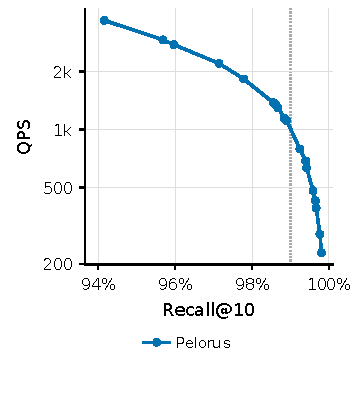
\includegraphics[width=0.8\linewidth]{pareto_openai_1536_1t.pdf}
  \caption{Measured \rquiver{} Recall@10--QPS frontier on {OpenAI-1536} ($990$K vectors, $1536$D, Zen~4, one query thread).}
  \label{fig:pareto_openai}
\end{figure}

\subsection{Comparison with Hyperbolic and Flat-Proxy Engines}
\label{subsec:eval_external}

\begin{table*}[t]
  \centering
  \caption{Measured comparison of \rquiver{} and baselines on {Cohere-1M} and {MERU-1M} (Zen~4, 32 build threads) at Recall@10 targets of $90\%$, $95\%$, $98\%$, $99\%$, and $99.5\%$. Panels (a) and (b) give main-sweep 1T and 24T QPS. The final block gives the independently tested log-map and quantized controls.}
  \label{tab:external_baselines}
  \footnotesize
  \setlength{\tabcolsep}{2pt}
  \begin{tabular}{@{}llrrrrrrrrr@{}}
\multicolumn{11}{@{}l}{\textbf{(a) Single-thread QPS}} \\
\toprule
\textbf{Dataset} & \textbf{Method} & \textbf{$M/L_c$} & \textbf{\shortstack{Build\\32T (s)}} & \textbf{\shortstack{Peak\\Rec@10}} & \textbf{$\ge90\%$} & \textbf{$\ge95\%$} & \textbf{$\ge98\%$} & \textbf{$\ge99\%$} & \textbf{$\ge99.5\%$} & \textbf{\shortstack{p99 (ms)\\at $99\%$}} \\
\midrule
Cohere-1M & Pelorus & 16/128 & 35.0 & 99.700\% & 4,939 & 4,939 & 2,907 & 1,930 & 738 & 0.62 \\
 & Faiss centered IP & 32/256 & 167.3 & 98.910\% & 1,652 & 830 & 127 & \missing & \missing & \missing \\
 & Faiss direction & 16/128 & 77.6 & 65.170\% & \missing & \missing & \missing & \missing & \missing & \missing \\
 & Faiss raw Lorentz-IP & 16/128 & 7.4 & 0.120\% & \missing & \missing & \missing & \missing & \missing & \missing \\
 & Milvus centered IP & 32/256 & 361.7 & 98.690\% & 252 & 238 & 76 & \missing & \missing & \missing \\
 & HDB FP32 dynamic & 32/256 & 414.8 & 96.780\% & 839 & 290 & \missing & \missing & \missing & \missing \\
 & HDB FP32 flat & 32/256 & 416.3 & 96.670\% & 946 & 279 & \missing & \missing & \missing & \missing \\
 & HDB FP64 dynamic & 32/256 & 866.5 & 94.430\% & 67 & \missing & \missing & \missing & \missing & \missing \\
 & HDB FP64 flat & 32/256 & 869.3 & 94.330\% & 74 & \missing & \missing & \missing & \missing & \missing \\
 & Exact-RobustPrune & 16/128 & 75.5 & 93.940\% & 629 & \missing & \missing & \missing & \missing & \missing \\
 & Polar-SQ8 & 16/128 & 66.9 & 99.780\% & 2,428 & 2,428 & 1,887 & 878 & 372 & 1.44 \\
 & Polar-FP32 & 16/128 & 190.2 & 99.783\% & 1,355 & 1,355 & 1,027 & 448 & 258 & 2.69 \\
\midrule
MERU-1M & Pelorus & 16/128 & 25.7 & 99.983\% & 5,846 & 4,521 & 2,547 & 2,547 & 1,669 & 0.50 \\
 & Faiss centered IP & 32/256 & 99.2 & 99.988\% & 4,312 & 2,800 & 1,903 & 1,059 & 872 & 1.43 \\
 & Faiss direction & 16/128 & 48.8 & 100.000\% & 3,460 & 1,814 & 1,480 & 1,078 & 1,078 & 1.30 \\
 & Faiss raw Lorentz-IP & 16/128 & 36.3 & 93.858\% & 841 & \missing & \missing & \missing & \missing & \missing \\
 & Milvus centered IP & 32/256 & 271.6 & 99.991\% & 297 & 297 & 297 & 260 & 233 & 5.30 \\
 & HDB FP32 dynamic & 16/128 & 86.5 & 99.947\% & 3,136 & 2,103 & 1,493 & 1,188 & 875 & 1.27 \\
 & HDB FP32 flat & 16/128 & 87.6 & 99.947\% & 3,187 & 2,184 & 1,579 & 1,296 & 966 & 1.15 \\
 & HDB FP64 dynamic & 32/256 & 631.4 & 99.955\% & 615 & 428 & 281 & 196 & 165 & 8.83 \\
 & HDB FP64 flat & 32/256 & 633.9 & 99.707\% & 480 & 320 & 186 & 93 & 46 & 21.68 \\
\bottomrule
\end{tabular}
\par\vspace{5pt}
\begin{tabular*}{\linewidth}{@{\extracolsep{\fill}}llrrrrr@{}}
\multicolumn{7}{@{}l}{\textbf{(b) 24-thread QPS (queries/s)}} \\
\toprule
\textbf{Dataset} & \textbf{Method} & \textbf{$\ge90\%$} & \textbf{$\ge95\%$} & \textbf{$\ge98\%$} & \textbf{$\ge99\%$} & \textbf{$\ge99.5\%$} \\
\midrule
Cohere-1M & Pelorus & 96,584 & 96,584 & 58,162 & 42,466 & 17,137 \\
 & Faiss centered IP & 10,717 & 10,717 & 1,660 & \missing & \missing \\
 & Faiss direction & \missing & \missing & \missing & \missing & \missing \\
 & Faiss raw Lorentz-IP & \missing & \missing & \missing & \missing & \missing \\
 & Milvus centered IP & 1,115 & 1,115 & 999 & \missing & \missing \\
 & HDB FP32 dynamic & 3,416 & 3,416 & \missing & \missing & \missing \\
 & HDB FP32 flat & 3,656 & 3,656 & \missing & \missing & \missing \\
 & HDB FP64 dynamic & \missing & \missing & \missing & \missing & \missing \\
 & HDB FP64 flat & \missing & \missing & \missing & \missing & \missing \\
 & Exact-RobustPrune & \missing & \missing & \missing & \missing & \missing \\
 & Polar-SQ8 & 46,034 & 46,034 & 34,639 & 16,844 & 7,016 \\
 & Polar-FP32 & 19,932 & 19,932 & 14,925 & 6,735 & 3,937 \\
\midrule
MERU-1M & Pelorus & 94,846 & 94,846 & 53,483 & 53,483 & 36,092 \\
 & Faiss centered IP & 33,189 & 33,189 & 22,488 & 13,005 & 9,349 \\
 & Faiss direction & 43,798 & 43,798 & 19,883 & 14,967 & 9,866 \\
 & Faiss raw Lorentz-IP & \missing & \missing & \missing & \missing & \missing \\
 & Milvus centered IP & 1,208 & 1,208 & 1,208 & 1,130 & 1,088 \\
 & HDB FP32 dynamic & 30,015 & 30,015 & 18,413 & 13,780 & 11,038 \\
 & HDB FP32 flat & 26,235 & 26,235 & 19,434 & 15,890 & 11,699 \\
 & HDB FP64 dynamic & 9,588 & 9,588 & 6,121 & 4,098 & 3,414 \\
 & HDB FP64 flat & 6,362 & 6,362 & 4,039 & 1,933 & 925 \\
\bottomrule
\end{tabular*}

  \par\smallskip
\begin{tabular*}{\linewidth}{@{\extracolsep{\fill}}lrrrrrr@{}}
\multicolumn{7}{@{}l}{\textbf{MERU-1M log-map and quantized controls ($99\%$ validation target, 10,000 test queries)}}\\
\toprule
& \multicolumn{3}{c}{1 thread} & \multicolumn{3}{c}{24 threads}\\
\cmidrule(lr){2-4}\cmidrule(l){5-7}
Method & Recall@10 (\%) & QPS & p99 (ms) & Recall@10 (\%) & QPS & p99 (ms)\\
\midrule
Faiss FP32 (log-map $L_2$) & 99.059 & 2,136 & 0.65 & 99.150 & 15,103 & 2.61\\
Faiss SQ8 (log-map $L_2$) & 99.119 & 1,220 & 1.07 & 99.119 & 26,786 & 1.28\\
Milvus SQ8 (centered IP) & 99.405 & 73 & 20.75 & 99.716 & 587 & 115.23\\
HDB SQ8 (Poincar\'e, FP64 rerank) & 99.224 & 763 & 1.85 & 99.224 & 13,620 & 2.52\\
Tangent 2-bit (paired engine) & 99.107 & 1,510 & 0.99 & 99.107 & 35,813 & 0.99\\
\rquiver{} 2-bit (paired engine) & 99.248 & 2,311 & 0.55 & 99.247 & 50,848 & 0.60\\
\bottomrule
\end{tabular*}

  \par\vspace{2pt}
  {\footnotesize \textit{Note:} HDB denotes HyperspaceDB. The paired-engine rows use a separate, sequentially timed comparison with validation-selected budgets. For \rquiver{}, $(L,B)$ is $(128,128)$ at 1T and $(128,32)$ at 24T. A dash denotes the absence of a qualifying measured point at that thread count. Build time and $M/L_c$ correspond to the fastest qualifying 1T configuration at $99\%$ recall, or the peak-recall configuration when $99\%$ is unreached. Each QPS column independently selects its fastest measured qualifying configuration. The $90\%$ and $95\%$ columns are selected from the existing measured configurations. Peak recall is the largest measured 1T recall; p99 is in milliseconds at the selected $99\%$ 1T point.}
\end{table*}

\begin{figure*}[t]
  \centering
  \begin{subfigure}[t]{0.485\textwidth}
    \centering
    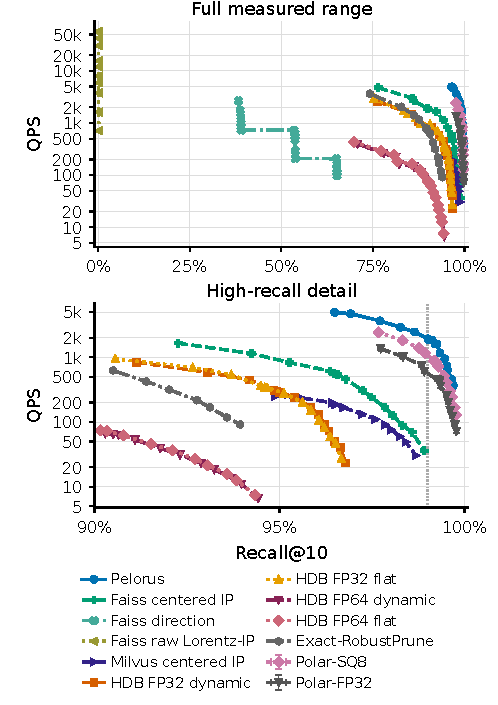
\includegraphics[width=\linewidth]{pareto_cohere_1m_1t.pdf}
    \caption{Cohere-1M ($768$D, 1 thread)}
    \label{fig:pareto_cohere}
  \end{subfigure}\hfill
  \begin{subfigure}[t]{0.485\textwidth}
    \centering
    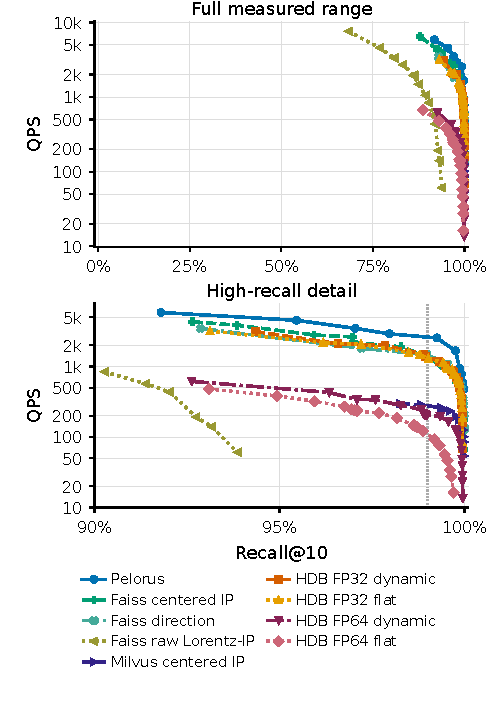
\includegraphics[width=\linewidth]{pareto_meru_1m_1t.pdf}
    \caption{MERU-1M ($512$D, 1 thread)}
    \label{fig:pareto_meru}
  \end{subfigure}
  \caption{Matched-dataset Recall@10--QPS frontiers of \rquiver{} and external baselines in the main Zen~4 sweep. Each panel shows the full measured recall range and a high-recall detail view. HDB denotes HyperspaceDB. Each method uses the first build per configuration (\S\ref{subsec:eval_setup}). Each method's frontier includes its measured build and search configurations; lines connect nondominated measurements.}
  \label{fig:real_pareto}
\end{figure*}

Table~\ref{tab:external_baselines} and Figure~\ref{fig:real_pareto} place \rquiver{} alongside {Exact-RobustPrune}~\cite{prokhorenkova2022hyperbolic}, {HDB} ({HyperspaceDB}~\cite{glukhota2026hyperspacedb}), and flat inner-product {HNSW} proxies in {Faiss}~\cite{douze2024faiss} ({Faiss centered IP}, {Faiss direction}, {Faiss raw Lorentz-IP}) and {Milvus}~\cite{wang2021milvus} ({Milvus centered IP}).
On the mapped {Cohere-1M} benchmark (Figure~\ref{fig:pareto_cohere}), \rquiver{} builds in $35.0$\,s, reaches $99.70\%$ peak Recall@10, and sustains $1{,}930$\,QPS (1T) and $42{,}466$\,QPS (24T) at $\ge 99\%$ recall.
On {Cohere-1M}, {Exact-RobustPrune} ($16/128$, $L\le2{,}048$) reaches $93.94\%$ peak Recall@10 ($75.5$\,s build), {HDB FP32 dynamic} and {HDB FP32 flat} ($32/256$) reach $96.78\%$ and $96.67\%$ ($414.8$\,s and $416.3$\,s build), and {HDB FP64 dynamic} and {HDB FP64 flat} ($32/256$) reach $94.43\%$ and $94.33\%$ ($866.5$\,s and $869.3$\,s); at the common $95\%$ recall target, \rquiver{} delivers $4{,}939$\,QPS (1T) and $96{,}584$\,QPS (24T) compared with $290$\,QPS (1T, $17.0\times$) and $3{,}416$\,QPS (24T, $28.3\times$) for {HDB FP32 dynamic}.
In the {Cohere-1M} flat {HNSW} sweeps ($ef\le4{,}096$), {Faiss centered IP} and {Milvus centered IP} ($32/256$) peak at $98.91\%$ and $98.69\%$ Recall@10 ($167.3$\,s and $361.7$\,s build; at $98\%$ recall, \rquiver{} attains $2{,}907$\,QPS on 1T and $58{,}162$\,QPS on 24T vs.\ $127$ / $1{,}660$\,QPS for {Faiss centered IP} and $76$ / $999$\,QPS for {Milvus centered IP}), while {Faiss direction} and {Faiss raw Lorentz-IP} reach $65.17\%$ and $0.12\%$. Under matched $M/L_c = 16/128$ ($ef \le 4{,}096$), external {Cohere-1M} peak recalls drop further to $93.84\%$/$93.64\%$ for {HDB FP32 dynamic/flat} ($106.1$\,s/$107.5$\,s build; $558$/$530$\,QPS 1T at $\ge 90\%$, missing $95\%$), $89.94\%$/$89.74\%$ for {HDB FP64}, and $97.93\%$/$97.99\%$ for {Faiss/Milvus centered IP} ($517$/$176$\,QPS 1T at $\ge 95\%$, missing $98\%$).

On {MERU-1M}, HDB FP32 flat reaches $1{,}296$/$15{,}890$\,QPS at $99.026\%$ recall and HDB FP32 dynamic reaches $1{,}188$/$13{,}780$ at $99.312\%$. At the $99\%$ target, \rquiver{} serves $1.97\times$/$3.37\times$ the HDB flat throughput (1T/24T).

\paragraph{SQ8 graph indices.}
On {MERU-1M}, HyperspaceDB SQ8 top-10 recall peaks at $63.93\%$ (Poincar\'e) and $51.75\%$ (Lorentz) across dynamic/flat layouts, $16/128$ and $32/256$ builds, and $ef\le4{,}096$. With the same cold FP32 vectors and $128$ candidates reranked in FP64, Poincar\'e SQ8 reaches $99.224\%$ at $763$/$13{,}620$\,QPS (1T/24T, $16/128$, $ef=256$). Lorentz SQ8 peaks at $96.66\%$ with this rerank budget.
Table~\ref{tab:official_sq8} evaluates Faiss \texttt{IndexHNSWSQ} on log-map $L_2$ and Milvus \texttt{HNSW\_SQ} on centered IP ($M/L_c=16/128$). At the $99\%$ validation target, Faiss serves $1{,}220/26{,}786$\,QPS at $99.119\%$ test recall (1T/24T). Milvus serves $73/587$\,QPS at $99.405/99.716\%$. Both systems test direct top-10 and FP64 geodesic reranking of 128 candidates. Faiss timings use the in-process C++ API. Milvus timings include the Python client and public gRPC call.

\begin{table}[!htbp]
 \centering
 \caption{MERU-1M with official SQ8 HNSW indices ($M/L_c=16/128$). For each target and thread count, $ef$ and $B$ are selected on 2,000 validation queries. Cells report outcomes on 10,000 test queries.}
 \label{tab:official_sq8}
 \footnotesize
 \setlength{\tabcolsep}{2.4pt}
 \begin{tabular}{@{}lrrrrrrr@{}}
 \toprule
 & Target & \multicolumn{3}{c}{One thread} & \multicolumn{3}{c}{24 threads}\\
 \cmidrule(lr){3-5}\cmidrule(lr){6-8}
 Engine & (\%) & R@10 (\%) & QPS & $p_{99}$ (ms) & R@10 (\%) & QPS & $p_{99}$ (ms)\\
 \midrule
Faiss & 98 & 98.463 & 1,961 & 0.74 & 98.463 & 41,457 & 0.88 \\
 & 99 & 99.119 & 1,220 & 1.07 & 99.119 & 26,786 & 1.28 \\
 & 99.5 & 99.578 & 973 & 1.37 & 99.578 & 20,805 & 1.65 \\
Milvus & 98 & 98.268 & 117 & 12.63 & 98.200 & 1,162 & 32.81 \\
 & 99 & 99.405 & 73 & 20.75 & 99.716 & 587 & 115.23 \\
 & 99.5 & 99.716 & 52 & 28.72 & 99.716 & 595 & 118.12 \\
 \bottomrule
 \end{tabular}
\end{table}


\paragraph{Tangent-space controls.}
Following {HyEm}'s candidate retrieval step~\cite{deng2026hyem}, we map $x$ to $\atanh(\|x\|)x/\|x\|$ (zero maps to zero). On {MERU-1M}, {Faiss} $L_2$ HNSW selects $M/L_c=16/128$ and $ef=128$ at both thread counts. Returning top-10 directly serves $2{,}136$\,QPS at $99.06\%$ recall on one thread. At 24 threads, FP64 geodesic reranking of 128 candidates serves $15{,}103$\,QPS at $99.15\%$. At the $99\%$ target, \rquiver{} serves $1.19\times$ and $3.54\times$ the FP32 log-map throughput at 1T and 24T, respectively. Each worker takes one query from a shared queue and searches single-threaded. On mapped {Cohere-1M}, log-map HNSW peaks at $86.42\%$ on its separate 500-query test subset.

We also compare the two navigation metrics inside the same Rust engine on {MERU-1M} (Table~\ref{tab:tangent_sm}). The tangent graph stores the log-map norm $t_v=\atanh(\|v\|)$ and the same 2-bit {SM} direction as \rquiver{}. It uses $(t_q-t_v)^2+2t_qt_v(1-\hat\gamma_{qv})$ for squared Euclidean distance in construction and beam search. Ordinary isotropic RobustPrune uses $\alpha=1.2$, fills unused slots by distance, and inserts vertices in input order. Search starts from one entry. Both graphs use $M_0=32$, $L_c=128$, the original FP32 vectors, and the same FP64 geodesic reranker.

We ran the two methods serially. Rayon distributed independent queries across workers. We warmed each condition with 200 queries. For each method and thread count, the first build selected the fastest $(L,B)$ reaching $99\%$ recall on 2,000 validation queries. We then measured the frozen settings on 10,000 disjoint test queries using the first build.

\begin{table*}[t]
  \centering
  \caption{MERU-1M tangent-space and native 2-bit graphs on the independent test queries. Each method uses its first build.}
  \label{tab:tangent_sm}
  \small
  \begin{tabular*}{\linewidth}{@{\extracolsep{\fill}}lrrrrrrrrrr@{}}
    \toprule
    & \multicolumn{5}{c}{1 thread} & \multicolumn{5}{c}{24 threads} \\
    \cmidrule(lr){2-6}\cmidrule(l){7-11}
    Method & $(L,B)$ & Recall@10 & QPS & p99 (ms) & RSS (MiB) & $(L,B)$ & Recall@10 & QPS & p99 (ms) & RSS (MiB) \\
    \midrule
    \multicolumn{11}{@{}l}{\emph{Fixed candidate and rerank budgets}} \\
  Tangent 2-bit & $(128,128)$ & 97.837\% & 2,326 & 0.644 & 2,605 & $(128,128)$ & 97.837\% & 55,121 & 0.660 & 2,609 \\
  \rquiver{} & $(128,128)$ & 99.248\% & 2,248 & 0.555 & 2,722 & $(128,128)$ & 99.248\% & 51,733 & 0.592 & 2,726 \\
    \midrule
    \multicolumn{11}{@{}l}{\emph{Validation-selected operating points}} \\
  Tangent 2-bit & $(256,128)$ & 99.107\% & 1,510 & 0.989 & 2,609 & $(256,128)$ & 99.107\% & 35,813 & 0.993 & 2,605 \\
  \rquiver{} & $(128,128)$ & 99.248\% & 2,311 & 0.548 & 2,725 & $(128,32)$ & 99.247\% & 50,848 & 0.599 & 2,722 \\
    \bottomrule
  \end{tabular*}
  \par
  {\footnotesize $B$ is the nominal rerank budget. When $B<L$, \textsc{CJ-Gate} can admit additional candidates in \rquiver{}. Rows are timed independently. RSS includes cold vectors.}
\end{table*}


With $L=B=128$, all candidates reach reranking. Single-thread throughput is similar, and Recall@10 is 1.411 percentage points higher for \rquiver{}. At the validation-selected $99\%$ target, the tangent graph doubles its beam width to 256. \rquiver{} sustains $1.53\times$ its throughput at 1T and $1.42\times$ at 24T, using $516.8$ versus $428.0$\,MB of hot navigation memory. Both graphs have 32 million edges per build. All million vertices are reachable from \rquiver{}'s entries, compared with $999{,}701$ from the tangent graph's entry.

\subsection{Multi-Threaded Scaling Efficiency}
\label{subsec:eval_scaling}

\begin{figure*}[t]
  \centering
  \begin{subfigure}[t]{0.485\linewidth}
    \centering
    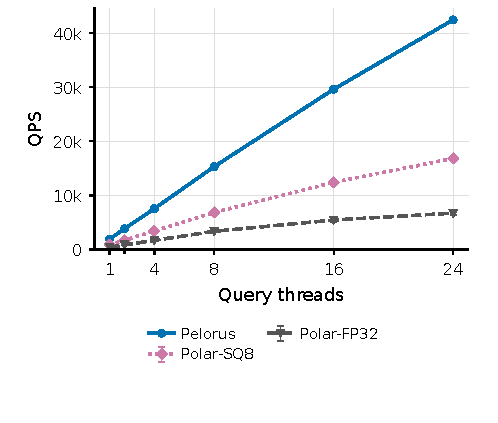
\includegraphics[width=\linewidth]{scaling_cohere_1m_r99.pdf}
    \caption{Cohere-1M ($\ge 99\%$ Recall)}
    \label{fig:scale_cohere}
  \end{subfigure}\hfill
  \begin{subfigure}[t]{0.485\linewidth}
    \centering
    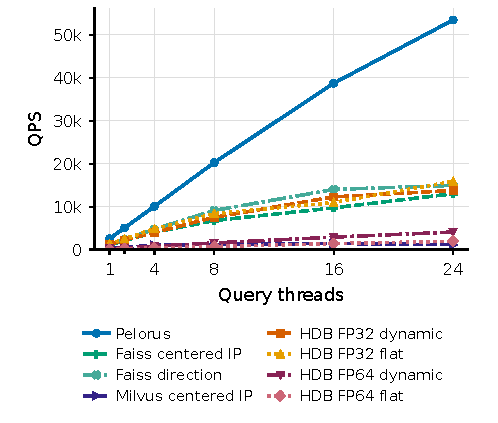
\includegraphics[width=\linewidth]{scaling_meru_1m_r99.pdf}
    \caption{MERU-1M ($\ge 99\%$ Recall)}
    \label{fig:scale_meru}
  \end{subfigure}
  \caption{Multi-threaded query scaling from 1 to 24 threads on Zen~4 at Recall@10 $\ge 99\%$. On {Cohere-1M}, \rquiver{} is compared against {Polar-SQ8} and {Polar-FP32} (external baseline peak recalls are reported in Table~\ref{tab:external_baselines}). On {MERU-1M}, \rquiver{} is compared against the main-sweep systems reaching $99\%$ recall. Each method selects its fastest qualifying configuration per thread count.}
  \label{fig:scaling}
\end{figure*}

Figure~\ref{fig:scaling} reports throughput scaling on the original sweep graph from $1$ to $24$ threads at $\ge 99\%$ Recall@10.
On {Cohere-1M} ($D=768$), the split-array and page layouts allocate $485.0$ and $517.0$\,MB of active navigation arrays, respectively (Table~\ref{tab:memory_audit}). Each page-layout slot holds a $64$\,B header including the sketch and $192$\,B of bitplanes. With read-only traversal, \rquiver{} scales by \textbf{$22.0\times$} at 24 threads on {Cohere-1M} ($1{,}930 \to 42{,}466$\,QPS, $91.7\%$ parallel efficiency; Figure~\ref{fig:scale_cohere}), \textbf{$21.0\times$} on {MERU-1M} ($2{,}547 \to 53{,}483$\,QPS), \textbf{$18.6\times$} on {OpenAI-1536} ($792 \to 14{,}731$\,QPS), and \textbf{$21.2\times$} on {WordNet-Hazy} ($3{,}089 \to 65{,}405$\,QPS).
By contrast, {Polar-FP32} reads $3{,}072$\,B ($48$ cache lines) per visited neighbor across a $3.37$\,GB footprint and scales by $15.3\times$ at 24 threads on {Cohere-1M} ($457 \to 7{,}004$\,QPS), widening \rquiver{}'s speedup from $4.23\times$ (1T) to \textbf{$6.06\times$ (24T)}; similarly, on {MERU-1M} (Figure~\ref{fig:scale_meru}), in-process FP32 systems scale by $11.6\times\text{--}12.3\times$ ({HDB FP32 dynamic/flat}: $1{,}188 \to 13{,}780$\,QPS and $1{,}296 \to 15{,}890$\,QPS; {Faiss centered IP}: $1{,}059 \to 13{,}005$\,QPS) and {Milvus centered IP} scales by $4.3\times$ ($260 \to 1{,}130$\,QPS), further widening \rquiver{}'s multi-threaded lead.

\subsection{Page Layout and Cold Storage}
\label{subsec:eval_storage}

With topology, code and query order fixed on the first {MERU-1M} builds, compact pages hold 21 vertices per page at $D=512$, up from 16. The allocated pages occupy $186.0$ versus $244.1$\,MiB. At $(L,B)=(128,64)$ both layouts return identical IDs and scores ($99.249\%$ recall). Single-thread throughput falls from $2{,}416$ to $2{,}305$\,QPS, while 24T rises from $47{,}470$ to $51{,}088$. On $65{,}536$-point probes derived from MERU, page allocations fall from $16.00$ to $10.24$\,MiB at $D=384$ and from $32.00$ to $21.34$\,MiB at $D=1024$. On $768$D {Cohere-1M}, both layouts occupy $244.1$\,MiB. At the same budget, compact pages serve $41{,}336$ versus $53{,}323$\,QPS at 24T. On $20$D {WordNet-Hazy}, compact pages use $6.43$ versus $10.25$\,MiB. Traversal can also share the cold FP32 vectors, eliminating separate code pages. Relative to the default pages, 1T process RSS falls from $70.5$ to $63.9$\,MiB. Recall rises from $97.340\%$ to $99.980\%$ while throughput falls from $4{,}578$ to $4{,}076$\,QPS.

The two layouts agree on returned IDs and scores at both measured budgets on every dimension. At $(256,128)$ on the first {Cohere-1M} build, compact and default pages reach $30{,}123/32{,}965$\,QPS at 24T with identical $99.260\%$ recall (Table~\ref{tab:layout_sweep}). Both layouts share a page translation per record. Packing also changes cache-line placement and address calculation. The container denied access to dTLB and LLC miss counters, so these timings measure the combined layout effect. Appendix~\ref{app:storage_measurements} reports both budgets, including process RSS and p99.

\begin{table}[t]
  \centering
  \caption{Cold reranking on {MERU-1M}. The 2-bit navigation graph stays in RAM. All rows use 24 threads, a 512\,MiB SSD cache and $\Delta_0=0.20$. The last column gives SSD bytes read per timed query in KiB.}
  \label{tab:meru_ssd}
  \footnotesize
  \setlength{\tabcolsep}{3pt}
  \begin{tabular}{@{}llrrrr@{}}
    \toprule
    Cold encoding & $L/B$ & Recall@10 & QPS & p99 (ms) & KiB/q \\
    \midrule
    FP32           & 512/128 & 99.917\% & 1,886 & 48.78 & 670.85 \\
    Cartesian FP16  & 512/128 & 99.902\% & 3,282 & 17.26 & 358.32 \\
    Polar FP16     & 512/128 & 99.902\% & 3,270 & 16.83 & 361.73 \\
    \midrule
    Centered SQ8    & 64/64 & 97.519\% & 23,760 & 4.48 & 44.31 \\
    Centered SQ4    & 64/64 & 90.123\% & 33,823 & 4.09 & 21.24 \\
    \bottomrule
  \end{tabular}
\end{table}

For SSD reranking we fix one graph, tune on $2{,}000$ queries, then time each condition once on $10{,}000$ test queries after 200 warmups. Batched \texttt{io\_uring} reads have a 32\,MiB in-flight budget. Polar FP16 and centered SQ4 retain an FP64 radius. At $L=512$, both FP16 formats nearly halve SSD traffic while retaining $99.902\%$ recall (Table~\ref{tab:meru_ssd}). At $L=64$, SQ4 reads $52\%$ fewer bytes per query than SQ8 and serves $42\%$ more queries per second at a cost of $7.396$ recall points. The highest SQ4 recall among the 43 configurations retested is $91.240\%$.

With cold FP32 and $99.917\%$ recall at 24T, moving from RAM to a 128\,MiB SSD cache cuts process RSS from $2.573$ to $0.825$\,GiB and throughput from $22{,}822$ to $1{,}308$\,QPS. At $(L,B)=(164,64)$, centered SQ8 returns the same top-10 results ($99.003\%$ recall) in RAM and with either cache. At 24T, RAM serves $51{,}040$\,QPS at $0.62$\,ms p99 and $1.155$\,GiB process RSS. Increasing the SSD cache from 128 to 512\,MiB cuts reads per query from $103.35$ to $10.00$, raises throughput from $2{,}749$ to $20{,}136$\,QPS, and lowers p99 from $23.87$ to $7.23$\,ms. RSS rises from $0.839$ to $1.228$\,GiB. Appendix~\ref{app:storage_measurements} lists 1T and 24T results for all five encodings with both cache budgets and RAM.
\subsection{Geometry and Execution Ablation Study}
\label{subsec:eval_ablation}

\begin{table}[t]
  \centering
  \caption{Controlled component ablations around {\rquiver{}-Core} on {Cohere-1M} (one thread, first build).}
  \label{tab:ablation_cohere}
  \small
  \setlength{\tabcolsep}{3pt}
  \begin{tabular}{@{}lrrrr@{}}
    \toprule
    & \textbf{Zero-In} & \textbf{Build} & \multicolumn{2}{c}{\textbf{1T QPS (p99 ms)}} \\
    \cmidrule(lr){4-5}
    \textbf{Variant} & \textbf{Islands} & \textbf{32T (s)} & \textbf{$\ge 99\%$} & \textbf{$\ge 99.5\%$} \\
    \midrule
    \textbf{\rquiver{}-Core} & 0 & 32.8 & 2,003 (0.59) & 687 (1.64) \\
    w/o \texttt{SymSketch256} & 0 & 32.8 & 1,850 (0.61) & 593 (1.97) \\
    w/o \texttt{HotSmPage} (SoA) & 0 & 32.8 & 1,701 (0.65) & 535 (2.14) \\
    SoA, \textsc{Stage-0.5} off & 0 & 32.8 & 1,665 (0.72) & 391 (2.83) \\
    SoA, Chord-Swap off & 521 & 32.4 & 1,739 (0.67) & 544 (2.06) \\
    \bottomrule
  \end{tabular}
\end{table}

\begin{figure*}[t]
  \centering
  \begin{subfigure}[t]{0.435\linewidth}
    \centering
    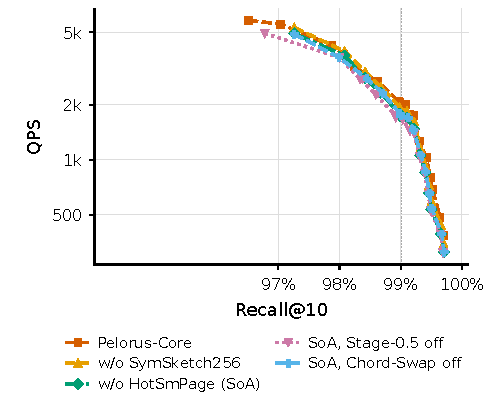
\includegraphics[width=\linewidth]{ablation_geometry_cohere_1m.pdf}
    \caption{Cohere-1M, topology and search}
    \label{fig:abl_geom}
  \end{subfigure}\hfill
  \begin{subfigure}[t]{0.435\linewidth}
    \centering
    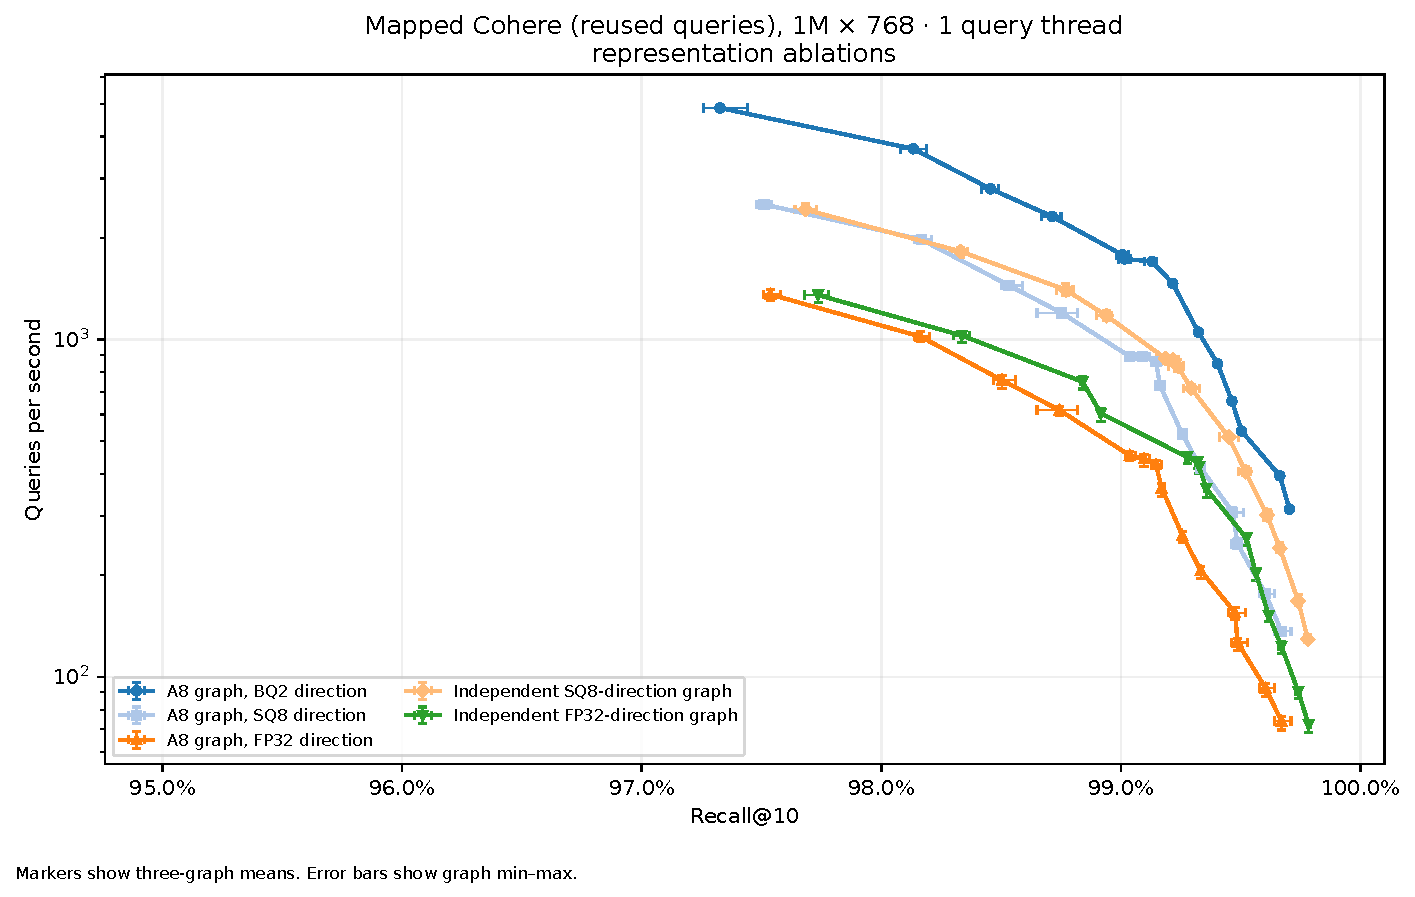
\includegraphics[width=\linewidth]{ablation_representation_cohere_1m.pdf}
    \caption{Cohere-1M, search representation}
    \label{fig:abl_repr}
  \end{subfigure}
  \par\smallskip
  \begin{subfigure}[t]{0.89\linewidth}
    \centering
    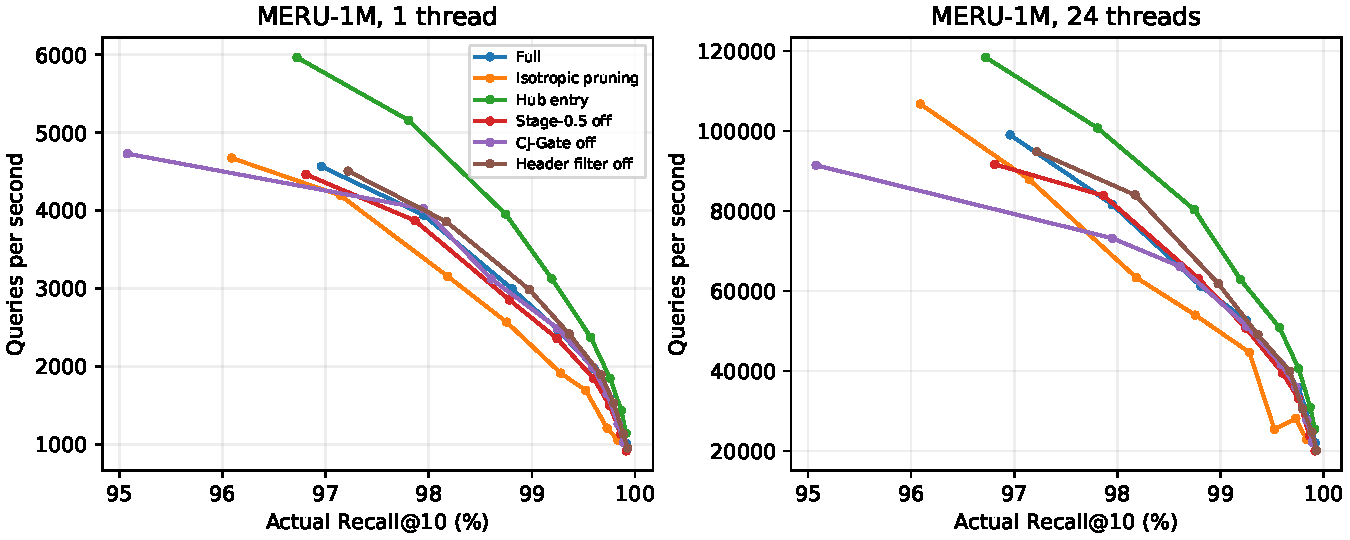
\includegraphics[width=\linewidth]{meru_ablation.pdf}
    \caption{MERU-1M, topology and search at eight fixed budgets.}
    \label{fig:abl_native}
  \end{subfigure}
  \caption{Component ablations on the first build. The upper panels give single-thread frontiers on {Cohere-1M}. The lower panels give measured recall and throughput at eight fixed budgets on {MERU-1M}.}
  \label{fig:ablation_pdf}
\end{figure*}
\begin{table}[t]
 \centering
 \caption{Pruning policies on Cohere-1M with the Core query engine. Fixed-budget Recall@10 uses $(L,B)=(192,64)$. Peak recall and the fastest 1T point reaching $99\%$ use the same 16 budgets for each policy ($L\le 2{,}048$). The final two rows are the first pair from an independent three-seed rebuild.}
 \label{tab:cohere_channels}
 \footnotesize
 \setlength{\tabcolsep}{3pt}
 \begin{tabular}{@{}lrrrrr@{}}
 \toprule
 & \multicolumn{2}{c}{Recall (\%)} & \multicolumn{3}{c}{$\ge 99\%$ Recall@10} \\
 \cmidrule(lr){2-3}\cmidrule(lr){4-6}
 Policy & Fixed & Peak & $L/B$ & QPS & p99 (ms)\\
 \midrule
All four channels & 99.00 & 99.70 & 192/64 & 1,957 & 0.58 \\
Geodesic off & 99.41 & 99.91 & 192/64 & 1,874 & 0.63 \\
Ring off & 97.09 & 98.74 & \missing & \missing & \missing \\
Inward elevator off & 99.08 & 99.73 & 192/64 & 1,928 & 0.61 \\
Outward elevator off & 99.00 & 99.65 & 208/64 & 1,972 & 0.58 \\
Both elevators off & 99.23 & 99.71 & 192/64 & 1,925 & 0.59 \\
Ring shield off & 98.99 & 99.69 & 200/64 & 1,896 & 0.62 \\
Earlier two-pass & 97.55 & 99.44 & 1536/64 & 426 & 2.64 \\
 \midrule
QuadriPrune (paired) & 98.97 & 99.72 & 200/64 & 1,946 & 0.60 \\
Angular quota (paired) & 98.93 & 99.87 & 208/64 & 1,721 & 0.68 \\
 \bottomrule
 \end{tabular}
\end{table}

\paragraph{Cohere-1M.}
The left and right Cohere panels in Figure~\ref{fig:ablation_pdf} use the first build in Table~\ref{tab:ablation_cohere}. The first varies topology and query decisions. The second holds the search policy in split-array form and changes the directional representation.
\begin{itemize}
  \item \emph{QuadriPrune.}
  The earlier two-pass policy first allocates up to $5M_0/8$ slots using directional-signature screening and a depth-adjusted geodesic dominance test. It fills the rest in order of signature distance plus a shell penalty, pruning within nearby shells before backfilling. For the observed {Cohere-1M} depth range $[0.98,3.39]$, the all-angle sufficient bound in Theorem~\ref{thm:vamana_pathologies}(1) extends at most to $(3.39-1.2\cdot0.98)/2.2\approx1.01$, below the first percentile of $1.45$. Beyond this sufficient bound, the theorem alone does not determine which candidates are occluded. Table~\ref{tab:cohere_channels} rebuilds each policy with the same seed and runs the same co-located Core engine, sketch, and reranker. QuadriPrune reaches $99\%$ at $L=192$, versus $1{,}536$ for the two-pass policy ($1{,}957$ versus $426$\,QPS). Removing the ring drops fixed-budget recall by $1.91$ points. Keeping the ring and allowing cross-shell occlusion changes recall by just $0.01$ points. Removing both elevators gives $99.23\%$ at the fixed budget and preserves full reachability on all three seeds. Removing either elevator also preserves the target, while removing the geodesic channel raises fixed-budget recall to $99.41\%$. Of the individual channel removals, only ring removal misses $99\%$ on all three seeds (peak $98.74$--$98.80\%$).

We also rebuilt QuadriPrune alongside a simpler graph for each of three seeds, alternating the run order. The simpler policy ranks candidates by two-bit angular loss and selects up to 16 of 32 neighbors by angular diversity ($\alpha=1.2$), with neither a shell shield nor dedicated geodesic or elevator passes. Both policies then use the same depth-aware refill, chord repair, entries and Core scoring. All six graphs reach every vertex with 32 million directed edges. In the first pair at the $99\%$ target, QuadriPrune serves $1{,}946$\,QPS at $99.08\%$ recall and the quota graph $1{,}721$ at $99.03\%$. At the $99.5\%$ target, the quota graph needs $L=384$ on all three builds ($1{,}057$--$1{,}064$\,QPS), while QuadriPrune needs $L=768$--$1{,}024$ ($638$--$786$\,QPS), all at $B=128$. Thus the throughput advantage on this shell changes direction with the recall target.
  \item \emph{\textsc{Stage-0.5} asymmetric refinement.}
  On the split-array path, ordering the pool by the calibrated hop score alone reduces $99.5\%$ throughput from $535$ to $391$\,QPS. At $99\%$ the two paths serve $1{,}701$ and $1{,}665$\,QPS.
  \item \emph{Spanning-Tree Chord-Swap Repair:}
  On the unrepaired build in this ablation, 521 vertices have zero in-degree and 530 are unreachable from the entry hub. Split-array throughput at $99\%$ is $1{,}739$\,QPS without repair and $1{,}701$ with it.
  \item \emph{\texttt{HotSmPage} and \texttt{SymSketch256}.}
  At $99\%$ recall, page co-location raises 1T throughput from $1{,}701$ to $1{,}850$\,QPS. Adding the sketch raises it to $2{,}003$\,QPS. At $99.5\%$ these configurations serve $535$, $593$ and $687$\,QPS.
\end{itemize}

A $2\times2$ query-side ablation holds the full Cohere graph, PolarRouter and six budgets fixed. Switching \textsc{CJ-Gate} preserves the IDs and scores for all $1{,}000$ queries at every budget. With the gate off, sketch-margin calibration at $(L,B,\Delta_0)=(192,64,0.12)$ moves recall from $99.00$ to $99.03\%$ and 1T throughput from $1{,}960$ to $1{,}800$\,QPS. At $(64,64,0.20)$ it moves recall from $98.15$ to $97.94\%$. At $(768,128,0.12)$ it moves recall from $99.49$ to $99.52\%$, making this smaller beam eligible at the highest target.

A separate entry comparison on one Cohere Core graph selects $L=512$ for PolarRouter and $768$ for hubs alone at a $99.5\%$ tuning target ($B=128$ for both). On the 500 held-out queries, PolarRouter reaches $99.30\%$ recall at $977/20{,}055$\,QPS (1T/24T), and hubs alone reach $99.20\%$ at $818/16{,}657$\,QPS. A separate header trace inspects 32 queries per seed. On Cohere the radial bound by itself rejects zero candidates. The default sketch test rejects $51.65\%$ of inspected candidates, falling to $45.82\%$ when the radial term is removed from that test.

\paragraph{MERU-1M.}
Figure~\ref{fig:abl_native} uses one graph for all query switches. The isotropic control rebuilds the graph with the same degree, refill and repair. It discards candidate $v$ at $u$ if a selected $p$ satisfies $\alpha\tilde d(p,v)\le\tilde d(u,v)$, where $\tilde d$ is the geodesic distance estimate recovered from the quantized proxy. At $L=B=128$, QuadriPrune raises recall from $98.755\%$ to $99.251\%$ ($2{,}568$ to $2{,}470$\,QPS, 1T). At $(256,128)$, hub-only entry serves $1{,}848$ versus $1{,}588$\,QPS for the full router ($99.757/99.754\%$ recall). Removing \textsc{Stage-0.5} or the header filter gives $33{,}206$ or $30{,}593$\,QPS at 24T versus $35{,}872$ for the full method. Disabling \textsc{CJ-Gate} gives $36{,}031$\,QPS and $99.729\%$ recall.

The eight search budgets are fixed before measuring the 10,000 native test queries. At $(256,128)$ the full method and hub-only entry serve $35{,}872$ and $40{,}594$\,QPS at 24T. In the MERU header trace the radial bound alone again rejects zero. The default and radial-term-removed sketch tests reject $50.03\%$ and $49.98\%$.

Table~\ref{tab:auto_entry} uses validation queries to choose between hubs and PolarRouter together with $(L,B)$ on a full graph, independently at each target and thread count. At each of the 14 budgets both entries use the same graph and reranker. MERU uses its usual validation and test sets, and Cohere uses the archived 500/500 split. MERU selects hubs at all six operating points. At the $99\%$ target, fixed PolarRouter reaches $99.250\%$ at $2{,}272/49{,}731$\,QPS, while automatic entry reaches $99.203/99.202\%$ at $2{,}868/64{,}786$\,QPS. Each automatic run returns exactly the IDs and scores of its selected fixed policy. Timing either policy once can change the throughput ordering: at the $99.5\%$ MERU target and 24T, automatic entry serves $38{,}842$\,QPS versus $40{,}175$ for fixed PolarRouter. The 16 hubs bypass both cone scans on shallow MERU. At the $99.5\%$ validation target on Cohere, 1T selects PolarRouter with $L=512$ (hubs require $768$), while 24T selects hubs. Held-out recall is $99.36\%$ and $99.22\%$, respectively.

\begin{table}[t]
\centering
\caption{Automatic entry selection for full \rquiver{}. On each validation set we choose the fastest qualifying combination of entry, $L$ and $B$ at each thread count. Recall and QPS are measured on held-out queries. H denotes hubs alone and P denotes PolarRouter.}
\label{tab:auto_entry}
\footnotesize
\setlength{\tabcolsep}{2.5pt}
\begin{tabular}{@{}lrrrrrrr@{}}
\toprule
& Target & \multicolumn{3}{c}{One thread} & \multicolumn{3}{c}{24 threads}\\
\cmidrule(lr){3-5}\cmidrule(lr){6-8}
Dataset & (\%) & Entry & R@10 (\%) & QPS & Entry & R@10 (\%) & QPS\\
\midrule
MERU-1M & 98 & H & 98.745 & 3,801 & H & 98.745 & 80,145 \\
 & 99 & H & 99.203 & 2,868 & H & 99.202 & 64,786 \\
 & 99.5 & H & 99.580 & 2,270 & H & 99.640 & 38,842 \\
Cohere-1M & 98 & H & 98.260 & 3,237 & H & 98.260 & 46,870 \\
 & 99 & H & 99.060 & 1,875 & H & 99.060 & 36,580 \\
 & 99.5 & P & 99.360 & 921 & H & 99.220 & 17,031 \\
\bottomrule
\end{tabular}
\end{table}


\paragraph{Pruning channels.}
Table~\ref{tab:pruning_controls} holds degree, refill and repair fixed. At $L=B=128$ on MERU and $(256,128)$ on HyperE WordNet, removing the geodesic channel changes recall by $+0.03$ and $-9.02$ points on the first build. On WordNet the other channel removals change recall by at most $0.32$ points. Ring width and elevator gap move recall by at most $0.43$ points across the tested settings. In the quota sweep all vertices remain reachable at 32 outgoing edges per vertex. The largest fixed-budget losses come from removing the ring on hollow-shell Cohere and geodesic edges on deep WordNet. Elevators supply cross-shell links within the fixed degree budget. On Cohere, removing both preserves the $99\%$ target.

\begin{table}[t]
  \centering
  \caption{QuadriPrune controls on shallow MERU and deep HyperE WordNet. Cells give Recall@10 (\%) on the first build. Each block has its own default.}
  \label{tab:pruning_controls}
  \footnotesize
  \setlength{\tabcolsep}{4pt}
  \begin{tabular}{@{}lrr@{}}
    \toprule
    Construction setting & MERU-1M & HyperE WordNet \\
    \midrule
  Default & 99.254 & 68.516 \\
  Geodesic off & 99.288 & 59.492 \\
  Ring off & 99.254 & 68.203 \\
  Inward elevator off & 99.255 & 68.555 \\
  Outward elevator off & 99.258 & 68.555 \\
  Ring width 0.30 & 99.254 & 68.945 \\
  Ring width 0.90 & 99.253 & 68.555 \\
  Elevator gap 0.09 & 99.252 & 68.672 \\
  Elevator gap 0.27 & 99.255 & 68.828 \\
    \midrule
    \multicolumn{3}{@{}l}{Geodesic and cumulative ring quotas (sixteenths)}\\
  6, 14 (default) & 99.251 & 68.555 \\
  4, 14 & 99.289 & 67.969 \\
  8, 14 & 99.207 & 68.945 \\
  6, 12 & 99.253 & 68.477 \\
  6, 15 & 99.255 & 68.711 \\
    \bottomrule
  \end{tabular}
\end{table}


\subsection{Synthetic Stress Tests, Recall-Loss Audit, and Applicability Boundaries}
\label{subsec:eval_synthetic}

\begin{table}[t]
  \centering
  \caption{Single-build sweep on synthetic extreme manifolds and real-manifold trade-offs on Zen~4 (complete \rquiver{} with tangent-cone rescue and adaptive \textsc{CJ-Gate} vs.\ \textbf{Global-SM} without cone rescue or \textsc{CJ-Gate}, $0$\,B/vertex overhead).}
  \label{tab:synthetic_rescue}
  \footnotesize
  \setlength{\tabcolsep}{1.7pt}
  \begin{tabular}{@{}lrrrrrr@{}}
    \toprule
    & \multicolumn{2}{c}{\textbf{Peak (\%)}} & & \multicolumn{3}{c}{\textbf{QPS at row target}} \\
    \cmidrule(lr){2-3}\cmidrule(lr){5-7}
    \textbf{Dataset (target)} & \textbf{\shortstack{Global\\SM}} & \textbf{\rquiver{}} & \textbf{Cones} & \textbf{\shortstack{Global\\SM 1T}} & \textbf{Full 1T} & \textbf{Full 24T} \\
    \midrule
    Clustered-Narrow & 34.220 & \textbf{99.945} & 256 & \emph{Unr.} & \textbf{1,840} & \textbf{38,876} \\
    Clustered-Wide & 73.865 & \textbf{99.995} & 256 & \emph{Unr.} & \textbf{2,704} & \textbf{57,144} \\
    Uniform-Wide ($98\%$) & 97.930 & \textbf{98.880} & 0 & \emph{Unr.} & $^\dagger$\emph{300} & $^\dagger$\emph{6,739} \\
    Uniform-Narrow & 62.410 & \textbf{64.735}$^\ddagger$ & 0 & \emph{Unr.} & \emph{Unr.} & \emph{Unr.} \\
    \midrule
    Cohere-1M ($99\%$) & 99.700 & \textbf{99.700} & 0 & \textbf{1,932} & 1,930 & 42,466 \\
    Cohere-1M ($99.5\%$) & 99.700 & \textbf{99.700} & 0 & 451 & \textbf{738} & \textbf{17,137} \\
    MERU-1M ($99\%$) & 99.952 & \textbf{99.983} & 0 & 1,443 & \textbf{2,547} & \textbf{53,483} \\
    MERU-1M ($99.5\%$) & 99.952 & \textbf{99.983} & 0 & 1,443 & \textbf{1,669} & \textbf{36,092} \\
    OpenAI-1536 ($99\%$) & 99.808 & \textbf{99.809} & 0 & \textbf{820} & 792 & 14,731 \\
    OpenAI-1536 ($99.5\%$) & 99.808 & \textbf{99.809} & 0 & \textbf{487} & 481 & 9,094 \\
    \bottomrule
  \end{tabular}
  \par\vspace{2pt}
  {\footnotesize\raggedright Peaks give 1T Recall@10. Unmarked rows have a $99\%$ throughput target. $^\dagger$At $\ge 98\%$ Recall@10 ($98.51\%$ at $L=1{,}536, B=128$; {Global-SM} caps at $97.93\%$). $^\ddagger$On the 32-query diagnostic probe, FP64 geodesic traversal on the same degree-32 graph visits and returns 199 of 320 true neighbors ($62.2\%$, $\mathcal{L}_{\mathrm{reach}}=37.8\%,\ \mathcal{L}_{\mathrm{beam}}=\mathcal{L}_{\mathrm{gate}}=0\%$), characterizing traversal loss on this constructed graph.\par}
\end{table}

\begin{table*}[t]
  \centering
  \caption{Measured comparison on all four synthetic distributions (1M vectors, 512D, Zen~4). Each QPS column selects the fastest measured configuration reaching its Recall@10 threshold. Panels (a) and (b) report one and 24 query threads.}
  \label{tab:synthetic_external}
  \footnotesize
  \setlength{\tabcolsep}{2pt}
  \begin{tabular}{@{}llrrrrrrrrr@{}}
\multicolumn{11}{@{}l}{\textbf{(a) Single-thread QPS}} \\
\toprule
\textbf{Dataset} & \textbf{Method} & \textbf{$M/L_c$} & \textbf{\shortstack{Build\\32T (s)}} & \textbf{\shortstack{Peak\\Rec@10}} & \textbf{$\ge90\%$} & \textbf{$\ge95\%$} & \textbf{$\ge98\%$} & \textbf{$\ge99\%$} & \textbf{$\ge99.5\%$} & \textbf{\shortstack{p99 (ms)\\at $99\%$}} \\
\midrule
Uniform-Narrow & Pelorus & 16/128 & 46.8 & 64.735\% & \missing & \missing & \missing & \missing & \missing & \missing \\
 & HDB FP32 flat & 32/256 & 478.2 & 92.170\% & 18 & \missing & \missing & \missing & \missing & \missing \\
 & Faiss centered IP & 32/256 & 311.3 & 29.860\% & \missing & \missing & \missing & \missing & \missing & \missing \\
 & Milvus centered IP & 32/256 & 573.6 & 46.445\% & \missing & \missing & \missing & \missing & \missing & \missing \\
\midrule
Uniform-Wide & Pelorus & 16/128 & 31.9 & 98.880\% & 639 & 397 & 300 & \missing & \missing & \missing \\
 & HDB FP32 flat & 32/256 & 299.6 & 97.860\% & 241 & 103 & \missing & \missing & \missing & \missing \\
 & Faiss centered IP & 32/256 & 140.1 & 48.640\% & \missing & \missing & \missing & \missing & \missing & \missing \\
 & Milvus centered IP & 32/256 & 255.1 & 54.040\% & \missing & \missing & \missing & \missing & \missing & \missing \\
\midrule
Clustered-Narrow & Pelorus & 16/128 & 25.3 & 99.945\% & 3,371 & 2,875 & 2,092 & 1,840 & 1,551 & 0.67 \\
 & HDB FP32 flat & 32/256 & 106.4 & 99.950\% & 1,568 & 1,315 & 1,133 & 998 & 998 & 1.33 \\
 & Faiss centered IP & 32/256 & 35.2 & 21.245\% & \missing & \missing & \missing & \missing & \missing & \missing \\
 & Milvus centered IP & 32/256 & 146.8 & 19.525\% & \missing & \missing & \missing & \missing & \missing & \missing \\
\midrule
Clustered-Wide & Pelorus & 16/128 & 19.4 & 99.995\% & 4,113 & 3,572 & 3,141 & 2,704 & 2,704 & 0.44 \\
 & HDB FP32 flat & 32/256 & 73.7 & 99.500\% & 1,037 & 908 & 735 & 735 & 645 & 2.14 \\
 & Faiss centered IP & 32/256 & 38.3 & 4.015\% & \missing & \missing & \missing & \missing & \missing & \missing \\
 & Milvus centered IP & 32/256 & 273.7 & 9.330\% & \missing & \missing & \missing & \missing & \missing & \missing \\
\bottomrule
\end{tabular}
\par\vspace{5pt}
\begin{tabular*}{\linewidth}{@{\extracolsep{\fill}}llrrrrr@{}}
\multicolumn{7}{@{}l}{\textbf{(b) 24-thread QPS (queries/s)}} \\
\toprule
\textbf{Dataset} & \textbf{Method} & \textbf{$\ge90\%$} & \textbf{$\ge95\%$} & \textbf{$\ge98\%$} & \textbf{$\ge99\%$} & \textbf{$\ge99.5\%$} \\
\midrule
Uniform-Narrow & Pelorus & \missing & \missing & \missing & \missing & \missing \\
 & HDB FP32 flat & 288 & \missing & \missing & \missing & \missing \\
 & Faiss centered IP & \missing & \missing & \missing & \missing & \missing \\
 & Milvus centered IP & \missing & \missing & \missing & \missing & \missing \\
\midrule
Uniform-Wide & Pelorus & 9,363 & 9,363 & 6,739 & \missing & \missing \\
 & HDB FP32 flat & 1,727 & 1,072 & \missing & \missing & \missing \\
 & Faiss centered IP & \missing & \missing & \missing & \missing & \missing \\
 & Milvus centered IP & \missing & \missing & \missing & \missing & \missing \\
\midrule
Clustered-Narrow & Pelorus & 55,231 & 55,231 & 44,175 & 38,876 & 33,132 \\
 & HDB FP32 flat & 17,024 & 17,024 & 14,483 & 13,311 & 13,311 \\
 & Faiss centered IP & \missing & \missing & \missing & \missing & \missing \\
 & Milvus centered IP & \missing & \missing & \missing & \missing & \missing \\
\midrule
Clustered-Wide & Pelorus & 72,780 & 72,780 & 70,801 & 57,144 & 57,144 \\
 & HDB FP32 flat & 15,090 & 15,090 & 12,519 & 12,519 & 12,011 \\
 & Faiss centered IP & \missing & \missing & \missing & \missing & \missing \\
 & Milvus centered IP & \missing & \missing & \missing & \missing & \missing \\
\bottomrule
\end{tabular*}

  \par\vspace{2pt}
  {\footnotesize \textit{Note:} The original sweep uses one graph and 32 build threads per configuration, $M/L_c=16/128$ and $L\le2{,}048$ for \rquiver{}, and $32/256$ and $ef\le4{,}096$ for external methods. It uses $2{,}000$ queries over five rounds. The additional Uniform-Narrow $32/256$ row uses the same test queries and $L$ through $4{,}096$. Both qualifying 24T cells select $L=4{,}096$ on the first build. A separate rebuild at $L=3{,}072$ served $1{,}572$\,QPS at $92.765\%$ recall. Peak recall is the largest measured 1T value. The p99 column uses the selected $99\%$-qualifying 1T point. A dash denotes the absence of a qualifying measured point for that thread count. Existing measured configurations supply the $90\%$ and $95\%$ selections.}
\end{table*}

\paragraph{External Comparisons Across Distributions.}
Table~\ref{tab:synthetic_external} reports all 12 external-baseline builds alongside \rquiver{} on the four synthetic distributions. On {Clustered-Narrow}, at Recall@10 $\ge99\%$, \rquiver{} reaches $1{,}840$\,QPS (1T) and $38{,}876$\,QPS (24T), compared with HDB FP32 flat at $998$ and $13{,}311$\,QPS ($1.84\times$ and $2.92\times$). Their selected points attain $99.385\%$ and $99.5\%$ recall, respectively. On {Clustered-Wide}, the corresponding rates are $2{,}704$/$57{,}144$ for \rquiver{} and $735$/$12{,}519$ for HDB ($3.68\times$/$4.56\times$), at $99.605\%$ and $99.495\%$ recall. These are common-threshold throughput comparisons across the reported construction budgets.
Centered Faiss and Milvus attain peak recalls of $21.245\%$/$19.525\%$ on {Clustered-Narrow} and $4.015\%$/$9.33\%$ on {Clustered-Wide}. On {Uniform-Wide}, peak recalls are $98.88\%$ for \rquiver{}, $97.86\%$ for HDB, $48.64\%$ for Faiss, and $54.04\%$ for Milvus. The {Uniform-Narrow} results expose a separate recall weakness of the current \rquiver{} configuration, analyzed below.

\paragraph{Four-Stage Telescoping Recall-Loss Audit.}
To pinpoint where candidates are lost on pathological manifolds, let $G_k(q)$ be the exact top-$k$ set, $V(q)$ the vertices visited during traversal, $C_L(q) \subseteq V(q)$ the retained beam pool of size $L$, $F_B(q) \subseteq C_L(q)$ the candidates admitted to exact reranking, and $R_k(q) \subseteq F_B(q)$ the returned top-$k$.
Because $R_k(q) \subseteq F_B(q) \subseteq C_L(q) \subseteq V(q)$, recall miss decomposes telescopically with zero overlap\ifpreprint\ (Appendix~\ref{app:loss_decomposition})\fi:
% 允许在召回分解公式前分页，避免跨栏浮动体挤压正文。
\begingroup
\predisplaypenalty=0
\begin{equation}
  \begin{aligned}
    &1 - \operatorname{Recall@}k(q) \\
    &= \underbrace{1 - \frac{|G_k \cap V|}{k}}_{\mathcal{L}_{\mathrm{reach}}(q)}
      + \underbrace{\frac{|G_k \cap (V \setminus C_L)|}{k}}_{\mathcal{L}_{\mathrm{beam}}(q)} \\
    &\quad+ \underbrace{\frac{|G_k \cap (C_L \setminus F_B)|}{k}}_{\mathcal{L}_{\mathrm{gate}}(q)}
      + \underbrace{\frac{|G_k \cap (F_B \setminus R_k)|}{k}}_{\mathcal{L}_{\mathrm{rerank}}(q)}.
  \end{aligned}
  \label{eq:four_stage_loss}
\end{equation}
\endgroup
For exact reranking on the coordinates defining the ground truth, the final term vanishes. A lossy cold store can change the final ordering.
On {Clustered-Narrow} ($L=256, B=128$), we traced 128 queries through {Global-SM} with residual coding and \textsc{CJ-Gate} disabled. Of $1{,}280$ true top-10 neighbors, traversal visited $1{,}202$ ($93.9\%$), the beam retained $631$ ($49.3\%$), and $422$ reached reranking and were returned ($33.0\%$). Across all $2{,}000$ queries, Recall@10 was $34.22\%$.
Increasing $L$ from $256$ to $2{,}048$ at fixed $B = 128$ monotonically \emph{lowers} {Global-SM} recall from $34.22\%$ ($2{,}071$\,QPS) through $31.78\%$ ($L=512$) and $29.43\%$ ($L=1{,}024$) down to $27.80\%$ ($L=2{,}048$) via intra-cluster pool dilution.

\paragraph{Synthetic Tangent-Cone Rescue and Real-Data Gate Gains.}
Both clustered datasets retain 256 cone axes. On {Clustered-Narrow} at $(L,B)=(256,128)$, {Global-SM} and full \rquiver{} attain $34.220\%$ and $99.385\%$ recall. The full method serves $1{,}840/38{,}876$\,QPS at 1T/24T and peaks at $99.945\%$ recall over the sweep. On {Clustered-Wide} at $(192,64)$, the corresponding recalls are $34.025\%$ and $99.605\%$, with $2{,}704/57{,}144$\,QPS for the full method. The peaks across budgets are $73.865\%$ and $99.995\%$, respectively (Table~\ref{tab:synthetic_rescue}).
Table~\ref{tab:synthetic_rescue} also reports {Global-SM} and full-method frontiers on the three million-scale real datasets, where both use global codes. At the $99.5\%$ target on {Cohere-1M}, the respective frontiers reach $451$ and $738$\,QPS. At the $99\%$ target on {MERU-1M} they reach $1{,}443$ and $2{,}547$\,QPS. Each frontier uses a separate build and its own measured budgets. The fixed-graph gate ablation in \S\ref{subsec:eval_ablation} isolates the effect of \textsc{CJ-Gate}.

On {Clustered-Narrow}, \textsc{CJ-Gate} on the global-code build saturates its budget $\bar B=\min(L,768)$ at $L=256,512,1{,}024$. On the residual-code build, it admits $128.8/129.2$ candidates on average at $L=256/384$ from $B_0=128$. At $(L,B_0)=(192,64)$ it raises recall from $97.695\%$ to $98.690\%$ and admits $120.7$ candidates.
On diffuse {Cohere-1M}, \textsc{CJ-Gate} admits a mean of $128.0$ candidates at $L=768$ ($736.8$ vs.\ $735.5$\,QPS with fixed $B=128$, $99.53\%$ recall). On native {MERU-1M} at $L=256$, its mean budget of $151.3$ matches full-pool ($B=256$) recall of $99.757\%$ at $35{,}833$ vs.\ $32{,}294$\,QPS (24T). Fixed $B=151$ attains $99.753\%$ and $35{,}546$\,QPS.

On a $32{,}768$-point mixture of equal parts tight cones and isotropic background at depths $3.9$--$4.1$, we hold the graph, hub entries and $(L,B)=(128,64)$ fixed. Scoring with residual rather than global codes on this graph raises recall from $82.34\%$ to $100.00\%$ on off-axis queries and from $72.30\%$ to $82.15\%$ on background queries (256 queries per group). On paired-cone controls, raising the mean purity threshold from $0.955$ to $0.98$ removes all axes. At the same 50\% mixture but $(L,B)=(256,128)$ the gain on off-axis queries narrows to $2.62$ points and the gain on background queries to $5.86$. At $(128,64)$, varying the clustered fraction from $25\%$ to $75\%$ changes the off-axis gain from $4.41$ to $24.77$ points. Each mixture has 64 generating axes in 64 dimensions, with the same 256 queries per group across mixtures. A separate fixed-coordinate control gives $96.45/96.25/96.48\%$ recall at $c=0.25/1/4$ against recomputed ground truth.

\paragraph{Degree-and-Budget Limits on Isotropic Narrow Shells.}
On {Uniform-Narrow} (1M points with uniform directions on $\mathbb{S}^{511}$, $\rho \in [3.9, 4.1]$, and local intrinsic dimensionality $\mathrm{LID} \approx 511$~\cite{houle2017lid}), \rquiver{} ($16/128, L\le2{,}048$) reaches $64.735\%$ recall ($62.41\%$ under {Global-SM}), whereas {HDB FP32 flat} ($32/256$) reaches $85.08\%$ at $ef=2{,}048$ and $92.17\%$ at $ef=4{,}096$ ($18$\,QPS 1T and $288$\,QPS 24T at $\ge 90\%$) on the full $2{,}000$-query test set, and {Faiss}/{Milvus} peak at $29.86\%$/$46.445\%$.
On a separate $32$-query probe over that same degree-32 \rquiver{} graph, exact FP64 geodesic search over FP32 coordinates returns 199 of 320 true neighbors ($62.2\%$ Recall@10, $\mathcal{L}_{\mathrm{reach}}=37.8\%,\ \mathcal{L}_{\mathrm{beam}}=\mathcal{L}_{\mathrm{gate}}=0\%$), locating these misses in the visited set at $L=2{,}048$ on the $16/128$ build. The graph is reachable from its entry hubs with an unrestricted traversal.
At matched $M/L_c=32/256$ ($M_0=64$, $772.8$\,MB hot), \rquiver{} builds in $147.5$\,s versus $478.2$\,s for {HDB}. At $L=3{,}072$ it reaches $92.525\%$ recall and $65.4$\,QPS at 1T. At $L=4{,}096$ recall reaches $95.285\%$ at $53.6$/$1{,}202$\,QPS.
Widening radial depth to $\rho \in [0.4, 6.0]$ ({Uniform-Wide}) enables exact polar radial lower-bound pruning (Proposition~\ref{prop:geodesic_apex}(1)) across shells and restores Recall@10 above $98\%$ (\textbf{$98.88\%$} peak, $300$\,QPS 1T and $6{,}739$\,QPS 24T at $98.51\%$).

\subsection{Residual Coding on Deep Native WordNet}
\label{subsec:eval_deep}
The published 10D {HyperE} embedding of WordNet hypernym relations~\cite{sala2018representation} has $p_{90}(\rho)=16.34$. After reserving 256 queries, the common representable database contains $73{,}258$ points. All three builds retain 33 cones. At $L=256,B_0=128$, first-build recall is $41.68\%$ with both dictionary and \textsc{CJ-Gate} off, $54.73\%$ with the dictionary alone, $54.14\%$ with the gate alone, and $68.67\%$ with both. The dictionary participates in graph construction. With the gate enabled, its paired gain is $14.53$ points ($95\%$ query-bootstrap interval $10.39$--$18.63$). Scoring the same outputs against source FP64 truth gives $53.28\%$ and $67.93\%$ recall, respectively.

\paragraph{Precision at the ball boundary.}
We recompute exact neighbors by exhaustive FP64 evaluation on both the published coordinates and the rounded representation. On the 256 benchmark queries the two exact top-10 lists share $2{,}503/2{,}560$ slots ($97.77\%$) on the common database. All $74{,}374$ distinct source rows lie inside the ball. Rounding the Cartesian coordinates to FP32 moves 752 points to or beyond the sphere, and 108 further rows collide with another in-ball row. The shared set has $73{,}514$ distinct points. Wider arithmetic in the reranker preserves only the information present in the stored vector.

\begin{table}[htbp]
  \centering
  \caption{HyperE WordNet conversion by source depth. Outside counts include the sphere. Duplicates count additional in-ball rows lost to FP32 collisions. Overlap is top-10 agreement with exhaustive source FP64 truth on the common database (64 queries per depth bin).}
  \label{tab:depth_precision}
  \footnotesize
  \setlength{\tabcolsep}{3pt}
  \begin{tabular}{@{}lrrrrr@{}}
  \toprule
  Depth & Source & Outside & Duplicates & FP32 overlap & Depth + direction \\
  \midrule
  $[0,8)$ & 10571 & 0 & 0 & 99.69\% & 99.69\% \\
  $[8,12)$ & 23800 & 0 & 0 & 98.12\% & 98.12\% \\
  $[12,16)$ & 30496 & 0 & 0 & 98.28\% & 99.38\% \\
  $[16,18)$ & 5973 & 1 & 1 & 92.50\% & 98.12\% \\
  $[18,20)$ & 2559 & 430 & 0 & 86.56\% & 96.25\% \\
  $[20,\infty)$ & 975 & 321 & 107 & 74.53\% & 86.41\% \\
  \bottomrule
  \end{tabular}
\end{table}


The fixed 256-query ANN split contains only five queries at depths $[18,20)$ and one at $\rho\ge20$. For the representation experiment we therefore draw 64 queries per depth bin from the shared set, remove all 384 from the database, and score exact top-10 overlap against the original FP64 ranking on the remaining points. Saving FP64 depth before rounding direction to FP32 improves the deepest bin from $74.53\%$ to $86.41\%$ overlap (Table~\ref{tab:depth_precision}). These neighbors come from exhaustive searches.\ifpreprint\ Appendix~\ref{app:wordnet_search} compares graph search and exact scanning on the original 256 queries.\fi
